\documentclass[10pt]{article}
\usepackage{tikz}
\usetikzlibrary{positioning,arrows}
\usetikzlibrary{shapes.geometric}
%\tikzstyle{v}=[draw, inner sep=6pt, minimum size=6pt, node distance=2.5cm]
\tikzstyle{w}=[draw, circle, inner sep=8pt, minimum size=6pt, node distance=2.5cm, fill = lightgray]
%\tikzstyle{ws}=[draw, circle, inner sep=6pt, minimum size=6pt, node distance=2.5cm, fill = lightgray]
\tikzstyle{u}=[draw, circle, inner sep=8pt, minimum size=6pt, node distance=2.5cm]

\begin{document}
\begin{figure}[h]
	\centering
	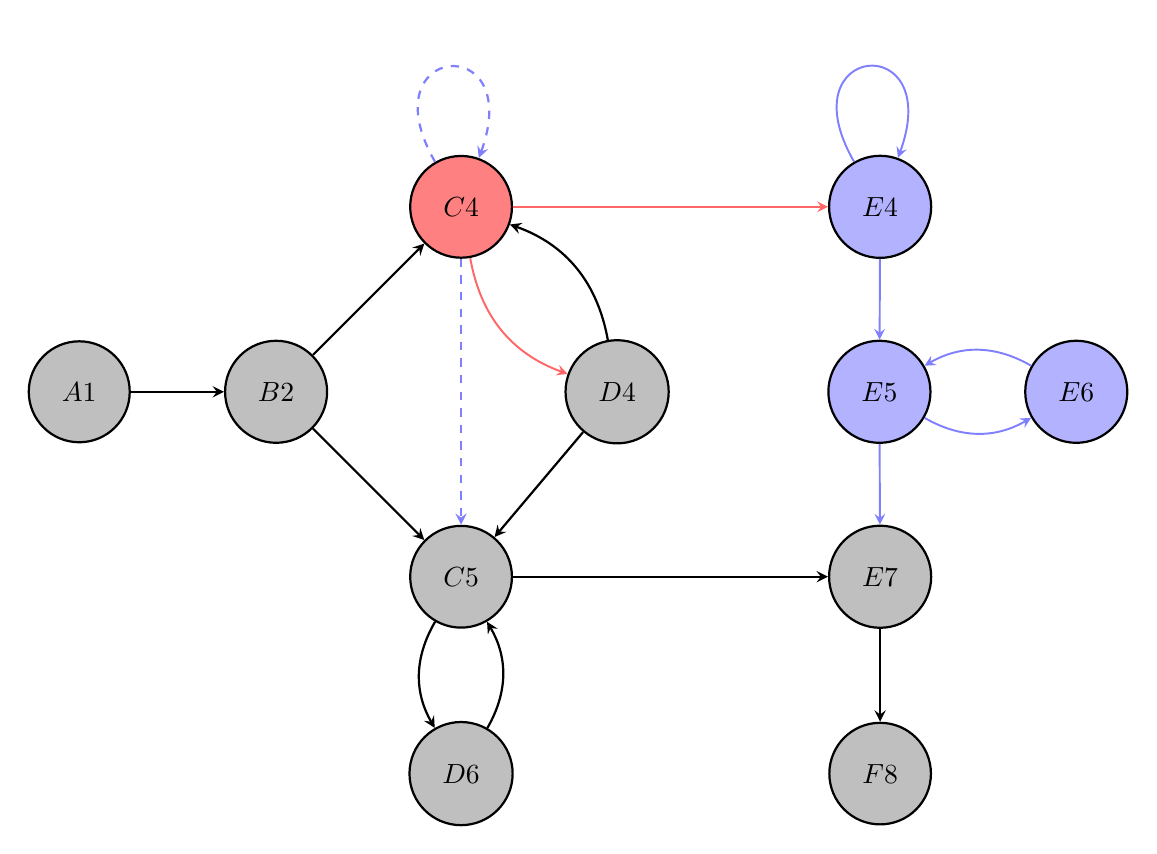
\begin{tikzpicture}[scale=1.0,transform shape, -triangle 45, thick]
	\node[w] (A1) at ( -6, 5) {$A1$}; 
	\node[w] (B2) [right of = A1] {$B2$};
	\node[w] (D4) [right = 3cm of B2] {$D4$};
	\node[u, fill=blue!30] (E5) [right = 2cm of D4] {$E5$};
	\node[u, fill=blue!30] (E6) [right of = E5] {$E6$};
	
	\node[u, fill=red!50] (C4) [above right =2cm of B2] {$C4$};
	\node[w] (C5) [below right =2cm of B2] {$C5$};
 	\node[w] (D6) [below of = C5] {$D6$};
	
 	\node[u, fill=blue!30] (E4) [right = 4cm of C4] {$E4$};
	\node[w] (E7) [right = 4cm of C5] {$E7$};
	\node[w] (F8) [below of = E7] {$F8$};
	
	\draw (A1) edge[->,>=stealth] (B2);
	\draw (B2) edge[->,>=stealth] (C4);
	\draw (B2) edge[->,>=stealth] (C5);
	\draw (C4) edge[->,>=stealth,color=blue!50, dashed] (C5);
	\draw (D4) edge[->,>=stealth] (C5);
	\draw (C4) edge[->,>=stealth,bend right, color=red!60, line width=.7pt] (D4);
	\draw (D4) edge[->,>=stealth,bend right] (C4);
	\draw (C5) edge[->,>=stealth,bend right] (D6);
	\draw (D6) edge[->,>=stealth,bend right] (C5);
	\draw (C4) edge[->,>=stealth,out=120,in=70,looseness=8, color=blue!50, dashed] (C4);
	\draw (C4) edge[->,>=stealth, color=red!60, line width=.7pt] (E4);
	\draw (C5) edge[->,>=stealth] (E7);
	\draw (E4) edge[->,>=stealth, color=blue!50, line width=.7pt] (E5);
	\draw (E5) edge[->,>=stealth, color=blue!50, line width=.7pt] (E7);
	\draw (E7) edge[->,>=stealth] (F8);
	\draw (E5) edge[->,>=stealth,bend right, color=blue!50, line width=.7pt] (E6);
	\draw (E6) edge[->,>=stealth,bend right, color=blue!50, line width=.7pt] (E5);
	\draw (E4) edge[->,>=stealth,out=120,in=70,looseness=8, color=blue!50, line width=.7pt] (E4);
	
	\end{tikzpicture}
  \label{fig:sat-reduction-edges}
\end{figure}
\end{document}
